\section{Introduction}

The CEBAF Large Acceptance Spectrometer for operation at 12 GeV beam energy (CLAS12)~\cite{clas12-nim} in
Hall~B at the Jefferson Laboratory (JLab) was designed to study electro-induced nuclear and hadronic reactions
by providing efficient detection of charged and neutral particles over a large fraction of the full solid angle. CLAS12
is based on two superconducting magnets and multiple detector subsystems that provide large coverage for the
detection of charged and neutral particles produced by the interaction of the electron beam from the JLab CEBAF
accelerator with a target located at the center of the spectrometer.

A six-coil torus magnet~\cite{magnets-nim} defines the six-sector structure of the so-called Forward Detector that
is outfitted with Drift Chambers~\cite{dc-nim} for charged particle tracking and multiple detector systems for
particle identification. These detectors include threshold Cherenkov Counters (which includes the Low Threshold
Cherenkov Counter and the High Threshold Cherenkov Counter~\cite{htcc-nim}) and Ring Imaging Cherenkov Counters
\cite{rich-nim}, scintillator-based time-of-flight hodoscopes~\cite{ftof-nim}, and electromagnetic calorimeters
\cite{ec-nim}. In the target region, a 5~T superconducting solenoid~\cite{magnets-nim} surrounds the Central Vertex
Tracker based on silicon and micromegas detectors~\cite{svt-nim,mm-nim}, and subsystems for particle identification
that include a time-of-flight scintillation counter barrel~\cite{ctof-nim} and a neutron detector~\cite{cnd-nim}, forming
the so-called Central Detector.

A model representation of the CLAS12 spectrometer identifying the Forward and Central Detectors is shown in
Fig.~\ref{fig:clas12-model}. In between the central and forward region, the CLAS12 Forward Tagger~\cite{ft-nim}
extends the kinematic coverage for the detection of electrons and photons at polar angles from 2$^\circ$ to 5$^\circ$.
The total number of readout channels of CLAS12 is larger than 100k. Typical trigger rates are 15~kHz. In 2018, data
rates of 500~MB/s with a live time of $>$95\% were achieved.

\begin{figure}
    \centering
    \includegraphics[width=1.0\columnwidth,keepaspectratio]{img/clas12-model.png}
    \caption{ Model representation of the CLAS12 spectrometer in Hall~B at JLab. The electron beam is incident from
      the left side of this figure. The CLAS12 detector is roughly 20~m in scale along the beam axis. The CLAS12
      Forward and Central Detectors are identified.}
    \label{fig:clas12-model}
\end{figure}

The spectrometer has met the performance criteria for operation at an instantaneous luminosity up to \cLuminosity
and momentum resolution $\sigma_p/p$ in the forward direction using the drift chambers and in the central direction
using the vertex tracker of $<$1\% and $<$3\%, respectively.

\subsection{LTCC Original Design and Performance}

The CLAS Cherenkov detector~\cite{Adams:2001kk} was instrumental in identifying electrons in the CLAS
spectrometer in Hall B during the Jefferson Lab 6~GeV era. It was used to provide electron/pion discrimination
with an efficiency $>$90\%.

The system consisted of identical detectors in each of the six sectors on the CLAS Forward Carriage, each
containing:

\begin{itemize}
	\item 108 lightweight adjustable mirrors;
	\item 36 Winston light collecting cones coated with p-terphenyl;
	\item 36 5-in Photonis X4500B PMTs;
	\item 36 passive magnetic shields;
	\item C$_4$F$_{10}$ gas, index of refraction: 1.00134.
\end{itemize}

The optics of each module was designed to focus the Cherenkov light onto a photomultiplier tube (PMT) associated
with that module and located in the region obscured by the CLAS torus magnet coils. Figure~\ref{fig:optics} shows
the optical arrangement of one module. The array of the modules in one sector is shown in \F{ltccArray}.

\begin{figure}[ht]
	\centering
	\includegraphics[width=1.0\columnwidth,keepaspectratio]{img/optics.png}
	\caption{Arrangement of one of the 216 modules of the CLAS Cherenkov detector, showing the optical and
          light collection components.}
	\label{fig:optics}
\end{figure}

\begin{figure}[ht]
	\centering
	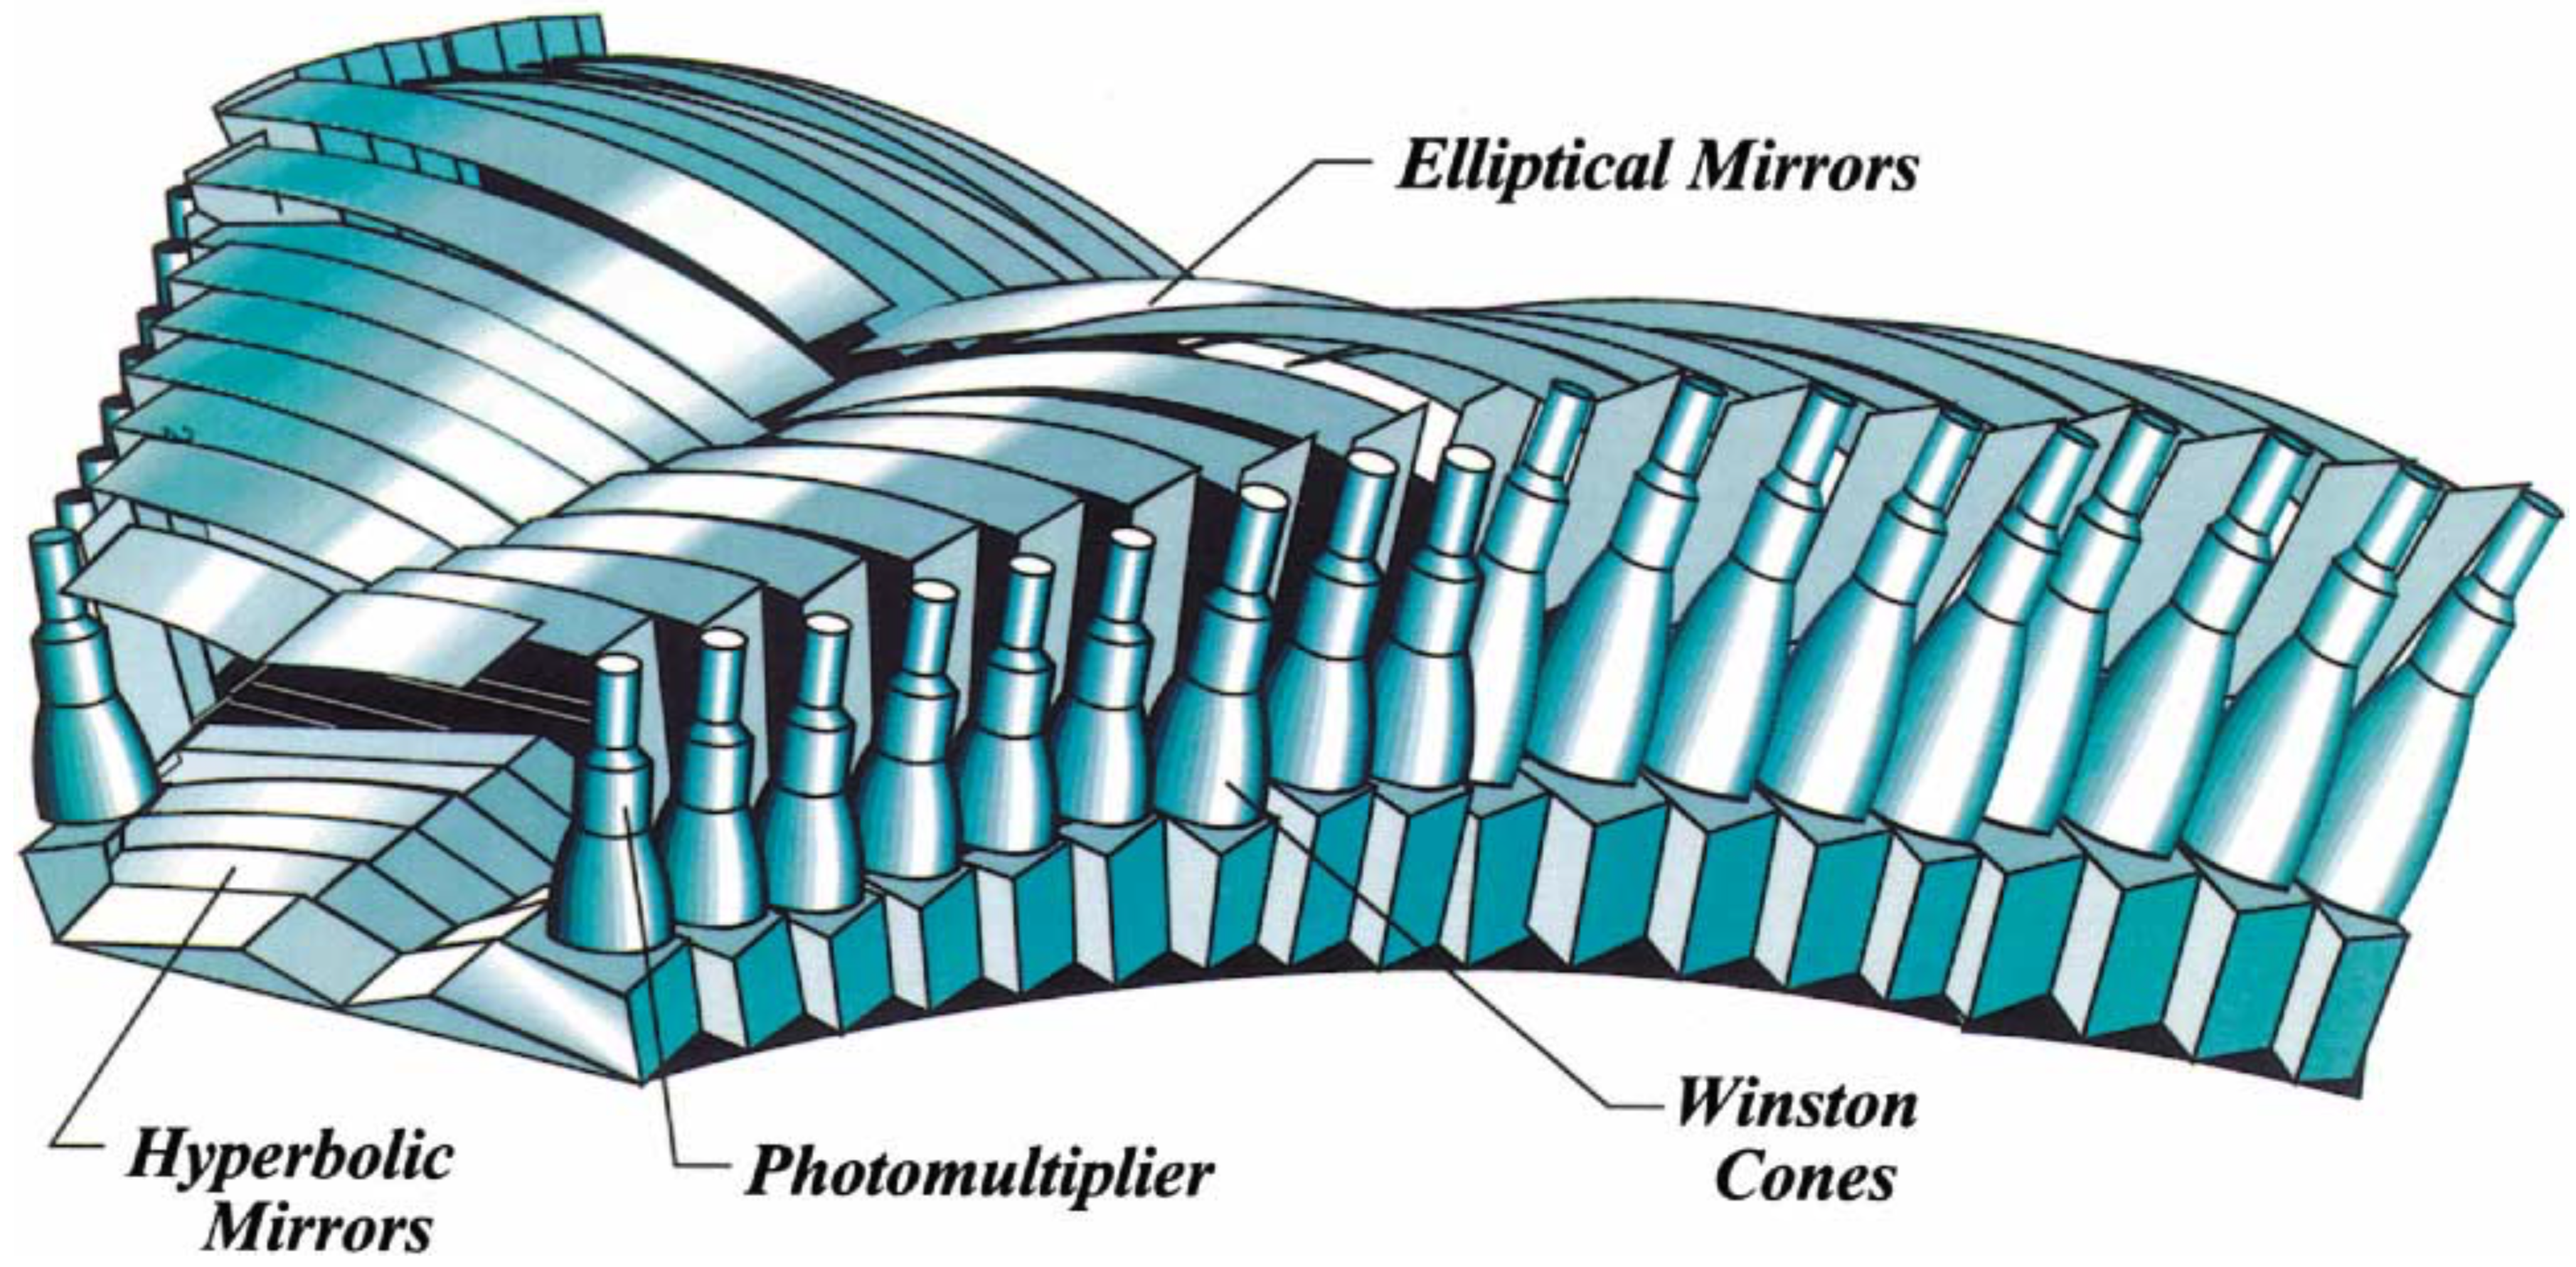
\includegraphics[width=1.0\columnwidth,keepaspectratio]{img/ltccArray.png}
	\caption{A diagram of the array of optical modules in one Cherenkov detector, highlighting
          the main system components.}
	\label{fig:ltccArray}
\end{figure}

The detector was operational for about 17~years. The typical number of photoelectrons detected for an electron
passing through the detector volume was between 10 and 20. The PMT nominal gain produced a signal too small
to be digitized by the CLAS12 readout ADC and TDC electronics and thus needed an additional $\times$10
multiplier module. The detector had several issues that affected the optics and system efficiency. It had 
significant gas leaks, the mirror misalignments led to inefficiencies that reduced the signal strength, and the
mirror supports were broken in several places in all sectors.

\subsection{Detector Upgrade}

With the 12~GeV energy upgraded accelerator~\cite{TDR12}, the momentum of the particles in Hall~B increases
substantially. Given the pion Cherenkov threshold of 2.6~GeV, the detector cannot provide a good electron/pion
discrimination for most energies and a new High Threshold Cherenkov Counter (HTCC)~\cite{htcc-nim} with a
CO$_2$ gas system has been built to provide electron discrimination up to momenta of 4.9~GeV.

\begin{table}[h]
    \small
	\begin{center}
        \begin{tabular}{ | p{5mm} | p{2.5mm} | p{2.5mm} | p{2.5mm} | p{2.5mm} | p{2.5mm} | p{2.5mm} | p{2.5mm} | p{2.5mm} | p{2.5mm} |p{2.5mm} |}
			\hline \hline
			 & 1 & 2 & 3 & 4 & 5 & 6 & 7 & 8 & 9 & 10      \\
			\hline
             e  & \cellcolor{grey} & \cellcolor{grey} & \cellcolor{grey}
                & \cellcolor{grey} & \cellcolor{grey} & \cellcolor{grey}
                & \cellcolor{grey} & \cellcolor{grey} & \cellcolor{grey} & \cellcolor{grey}  \\
         $\pi$  &  &  &
                & \cellcolor{grey} & \cellcolor{grey} & \cellcolor{grey}
                & \cellcolor{grey} & \cellcolor{grey} & \cellcolor{grey} & \cellcolor{grey}  \\
             k  & & & & & & &
                & \cellcolor{grey} & \cellcolor{grey} & \cellcolor{grey} \\
			\hline \hline
		\end{tabular}
	\end{center}
	\caption{The momentum coverage of the refurbished LTCC to provide for charged pion/kaon discrimination.
        The top row indicates the particle momenta in GeV. The highlighted boxes indicate the range for which particles
        produce a signal in the LTCC. The pion/kaon discrimination is provided from about 3.7 to 8.5~GeV.}
        \label{tab:newScope}
\end{table}

The heavier C$_4$F$_{10}$ gas can still be used to discriminate pions from kaons (see Table~\ref{tab:newScope}),
thus the detector was refurbished to a Low Threshold Cherenkov Counter (LTCC). The individual detector modules
have been modified to:

\begin{itemize}
	\item Support the new scope of pion/kaon discrimination;
	\item Address the gas leaks and other hardware issues.
\end{itemize}
